% --- Page Style ---
\settasks{label-width=4.6em, item-indent=4.6em}
\pagestyle{fancy}
\fancyhf{}
\lhead{Algebra --- Unit 6}
\rhead{Exam ID: \underline{\hspace{2cm}}}
\lfoot{All answers must be simplified. No calculators.}
\rfoot{Page \thepage}
\renewcommand{\headrulewidth}{0.4pt}
\renewcommand{\footrulewidth}{0.4pt}

% --- Header spanning both columns ---
\twocolumn[
  \begin{center}
    {\huge \textbf{Unit 6 Assessment}} \\
    \vgap
    {\large \textbf{Algebra}} \\
    \vgap
    \begin{tabular}{|l|l|}
      \hline
      \textbf{Student Name:} & \hspace{6cm} \\ \hline
      \textbf{Date:} & \hspace{6cm} \\ \hline
    \end{tabular}
  \end{center}
  \vgap
  \textbf{Instructions:} All answers must be simplified and exact. No calculators are allowed.
  \vgap
]

% % --- Form A ---
% \section*{Form A}

% \begin{enumerate}[leftmargin=*, label=\textbf{\arabic*.}]

%   \item Convert $\dfrac{4\pi}{9}$ to degrees. \points{1}
%   \vgap

%   \item Convert $600^{\circ}$ to radians. \points{1}
%   \vgap

%   \item Find two coterminal angles (one positive, one negative) for $\dfrac{3\pi}{7}$. \points{1}

%   Positive: \blank

%   Negative: \blank
%   \vgapp

%   \item Sketch each angle and state the quadrant (or axis) in which the terminal side lies. \points{3}

%   $-\dfrac{3\pi}{8}$: Quadrant: \blank

%   5 radians: Quadrant: \blank
%   \vgapp

%   \item Determine the reference angle for each. Your answer should match the form given. \points{1}

%   $-115^{\circ}$: \blank

%   $\dfrac{9\pi}{7}$: \blank

%   $\dfrac{19\pi}{8}$: \blank
%   \vgappp

%   \item Find the exact values of $x$ and $y$ in the diagram shown. \points{2}

%   \begin{center}
%   \begin{tikzpicture}[scale=0.55, line cap=round, line join=round]
%     % Right triangle: angle pi/6 at origin, hypotenuse 6
%     \draw[thick] (0,0) -- (5.196,0) -- (5.196,3) -- cycle;
%     \draw (5.196,0) rectangle (4.9,0.3);
%     \draw (0,0) ++(0:0.55) arc (0:30:0.55);
%     \node[right] at (5.196,1.5) {$y$};
%     \node[above] at (2.6,0) {$x$};
%     \node at (0.75,0.2) {\scriptsize $\frac{\pi}{6}$};
%     \node[above, sloped] at (2.6,1.5) {\scriptsize 6};
%   \end{tikzpicture}
%   \end{center}

%   $x = $ \blank

%   $y = $ \blank
%   \vgappp

%   \item A car drives in a circular pattern on a track with radius 800 feet. A central angle with measure $\dfrac{13\pi}{10}$ corresponds to the car's position after 40 seconds. What is the car's average velocity (in feet per second) over the first 40 seconds? Write your answer as an exact value in simplest form. \points{3}
%   \vgappp

%   \item Which of the following angles have the same reference angle? Select all that apply. \points{2}

%   \begin{tasks}(1)
%     \task $\dfrac{7\pi}{6}$
%     \task $\dfrac{11\pi}{4}$
%     \task $-\dfrac{16\pi}{6}$
%     \task $740^{\circ}$
%     \task $-\dfrac{19\pi}{9}$
%     \task $\dfrac{20\pi}{18}$
%     \task $\dfrac{5\pi}{7}$
%     \task $400^{\circ}$
%   \end{tasks}
%   \vgapp

%   \item Evaluate each trigonometric expression. \points{1}

%   \begin{center}
%   \small
%   \begin{tabular}{|l@{\quad}l|}
%   \hline
%   $\sin(90^{\circ})$: & \blank[3em] \\
%   $\sec(300^{\circ})$: & \blank[3em] \\
%   $\tan(5\pi/4)$: & \blank[3em] \\
%   $\csc(-\pi/6)$: & \blank[3em] \\
%   $\cos(-135^{\circ})$: & \blank[3em] \\
%   $\sec(225^{\circ})$: & \blank[3em] \\
%   $\cos(11\pi/4)$: & \blank[3em] \\
%   $\cot(5\pi/2)$: & \blank[3em] \\
%   $\sin(-5\pi/3)$: & \blank[3em] \\
%   \hline
%   \end{tabular}
%   \end{center}
%   \vgapp

%   \item If $\tan(\theta) = \dfrac{2}{9}$ and $\sec(\theta) < 0$, what is $\sin(\theta)$? \points{2}
%   \vgappp

%   \item Put the following in order from least to greatest. \points{3}

%   $\sin\bigl(\dfrac{8\pi}{3}\bigr),\ \cos(7\pi),\ \cos(10\pi),\ \cos\bigl(-\dfrac{5\pi}{3}\bigr),\ \tan\bigl(\dfrac{\pi}{6}\bigr),\ \cos\bigl(\dfrac{\pi}{13}\bigr)$

%   \begin{center}
%   \begin{tikzpicture}[x=0.5cm, line cap=round, line join=round]
%     \draw[thick,->] (-4,0) -- (4,0);
%     \foreach \k in {-3,-2,...,3} \draw (\k,2pt) -- (\k,-2pt);
%     \node[below] at (-4,-0.35) {Least};
%     \node[below] at (4,-0.35) {Greatest};
%   \end{tikzpicture}
%   \end{center}
%   \vgapp

%   \item \textbf{Part 1:} Fill in the first quadrant of the unit circle. For each angle, give both degrees and radians and the ordered pair $(x,y)$. \points{3}

%   \begin{center}
%   \begin{tikzpicture}[scale=1.1, line cap=round, line join=round]
%     \draw[thick] (0,0) circle (1.4);
%     \draw[thick,->] (-0.1,0) -- (1.6,0) node[right] {$x$};
%     \draw[thick,->] (0,-0.1) -- (0,1.6) node[above] {$y$};
%     \foreach \a in {0,30,45,60,90} {
%       \draw[gray] (0,0) -- (\a:1.5);
%     }
%     \node[below left] at (0,0) {$O$};
%     \node at (1.55,0) [right,font=\scriptsize] {$0$};
%     \node at (0,1.55) [above,font=\scriptsize] {$\frac{\pi}{2}$};
%   \end{tikzpicture}
%   \end{center}
%   \vgap

%   \item \textbf{Part 2:} If $\sin(\theta) = 0.915$ (assume $\theta$ in degrees), find: \points{1}

%   \begin{tasks}(1)
%     \task $\sec(90^{\circ} - \theta)$: \blank
%     \task $\sin(-\theta)$: \blank
%     \task $\cos(\theta - 90^{\circ})$: \blank
%     \task $\csc(\theta)$: \blank
%   \end{tasks}
%   \vgapp

% \end{enumerate}

% \clearpage
% % --- Form B ---
% \section*{Form B}

% \begin{enumerate}[leftmargin=*, label=\textbf{\arabic*.}, resume]

%   \item Convert $\dfrac{7\pi}{10}$ to degrees. \points{1}
%   \vgap

%   \item Convert $500^{\circ}$ to radians. \points{1}
%   \vgap

%   \item Find two coterminal angles (one positive, one negative) for $\dfrac{7\pi}{5}$. \points{1}

%   Positive: \blank

%   Negative: \blank
%   \vgapp

%   \item Sketch each angle and state the quadrant (or axis). \points{3}

%   $-\dfrac{5\pi}{8}$: Quadrant: \blank

%   3 radians: Quadrant: \blank
%   \vgapp

%   \item Determine the reference angle for each (match the form given). \points{1}

%   $-105^{\circ}$: \blank

%   $\dfrac{10\pi}{9}$: \blank

%   $\dfrac{21\pi}{8}$: \blank
%   \vgappp

%   \item Find the exact values of $x$ and $y$ in the diagram shown. \points{2}

%   \begin{center}
%   \begin{tikzpicture}[scale=0.6, line cap=round, line join=round]
%     % Right triangle: angle pi/4 at origin, hypotenuse 5
%     \draw[thick] (0,0) -- (3.536,0) -- (3.536,3.536) -- cycle;
%     \draw (3.536,0) rectangle (3.24,0.3);
%     \draw (0,0) ++(0:0.5) arc (0:45:0.5);
%     \node[right] at (3.536,1.77) {$y$};
%     \node[above] at (1.77,0) {$x$};
%     \node at (0.55,0.25) {\scriptsize $\frac{\pi}{4}$};
%     \node[above, sloped] at (1.77,1.77) {\scriptsize 5};
%   \end{tikzpicture}
%   \end{center}

%   $x = $ \blank

%   $y = $ \blank
%   \vgappp

%   \item A car drives on a circular track with radius 400 feet. A central angle of $\dfrac{13\pi}{20}$ corresponds to 40 seconds. What is the car's average velocity (ft/s) over the first 40 seconds? Exact value, simplest form. \points{3}
%   \vgappp

%   \item Which angles have the same reference angle? Select all that apply. \points{2}

%   \begin{tasks}(1)
%     \task $-\dfrac{19\pi}{9}$
%     \task $\dfrac{7\pi}{6}$
%     \task $740^{\circ}$
%     \task $\dfrac{20\pi}{18}$
%     \task $400^{\circ}$
%     \task $\dfrac{5\pi}{7}$
%     \task $\dfrac{11\pi}{4}$
%     \task $-\dfrac{16\pi}{6}$
%   \end{tasks}
%   \vgapp

%   \item Evaluate each trigonometric expression. \points{1}

%   \begin{center}
%   \small
%   \begin{tabular}{|l@{\quad}l|}
%   \hline
%   $\sin(270^{\circ})$: & \blank[3em] \\
%   $\sec(330^{\circ})$: & \blank[3em] \\
%   $\tan(3\pi/4)$: & \blank[3em] \\
%   $\csc(-\pi/3)$: & \blank[3em] \\
%   $\cos(135^{\circ})$: & \blank[3em] \\
%   $\sec(-225^{\circ})$: & \blank[3em] \\
%   $\cos(7\pi/4)$: & \blank[3em] \\
%   $\cot(9\pi/2)$: & \blank[3em] \\
%   $\sin(-5\pi/6)$: & \blank[3em] \\
%   \hline
%   \end{tabular}
%   \end{center}
%   \vgapp

%   \item If $\tan(\theta) = \dfrac{2}{7}$ and $\sec(\theta) < 0$, what is $\sin(\theta)$? \points{2}
%   \vgappp

%   \item Put in order from least to greatest. \points{3}

%   $\sin\bigl(\dfrac{7\pi}{3}\bigr),\ \cos(21\pi),\ \cos(12\pi),\ \cos\bigl(-\dfrac{5\pi}{3}\bigr),\ \tan\bigl(\dfrac{\pi}{6}\bigr),\ \cos\bigl(\dfrac{\pi}{13}\bigr)$

%   \begin{center}
%   \begin{tikzpicture}[x=0.5cm, line cap=round, line join=round]
%     \draw[thick,->] (-4,0) -- (4,0);
%     \foreach \k in {-3,-2,...,3} \draw (\k,2pt) -- (\k,-2pt);
%     \node[below] at (-4,-0.35) {Least};
%     \node[below] at (4,-0.35) {Greatest};
%   \end{tikzpicture}
%   \end{center}
%   \vgapp

%   \item \textbf{Part 1:} Fill in the first quadrant of the unit circle (degrees, radians, $(x,y)$). \points{3}

%   \begin{center}
%   \begin{tikzpicture}[scale=1.1, line cap=round, line join=round]
%     \draw[thick] (0,0) circle (1.4);
%     \draw[thick,->] (-0.1,0) -- (1.6,0) node[right] {$x$};
%     \draw[thick,->] (0,-0.1) -- (0,1.6) node[above] {$y$};
%     \foreach \a in {0,30,45,60,90} { \draw[gray] (0,0) -- (\a:1.5); }
%     \node[below left] at (0,0) {$O$};
%   \end{tikzpicture}
%   \end{center}
%   \vgap

%   \item \textbf{Part 2:} If $\sin(\theta) = -0.715$ ($\theta$ in degrees), find: \points{1}

%   \begin{tasks}(1)
%     \task $\sec(90^{\circ} - \theta)$: \blank
%     \task $\sin(-\theta)$: \blank
%     \task $\cos(\theta - 90^{\circ})$: \blank
%     \task $\csc(\theta)$: \blank
%   \end{tasks}
%   \vgapp

% \end{enumerate}

% \clearpage
% % --- Form C ---
% \section*{Form C}

% \begin{enumerate}[leftmargin=*, label=\textbf{\arabic*.}, resume]

%   \item Convert $\dfrac{7\pi}{12}$ to degrees. \points{1}
%   \vgap

%   \item Convert $490^{\circ}$ to radians. \points{1}
%   \vgap

%   \item Find two coterminal angles (one positive, one negative) for $\dfrac{3\pi}{11}$. \points{1}

%   Positive: \blank

%   Negative: \blank
%   \vgapp

%   \item Sketch each angle and state the quadrant (or axis). \points{3}

%   $-\dfrac{5\pi}{8}$: Quadrant: \blank

%   7 radians: Quadrant: \blank
%   \vgapp

%   \item Determine the reference angle for each (match the form given). \points{1}

%   $-100^{\circ}$: \blank

%   $\dfrac{11\pi}{9}$: \blank

%   $\dfrac{23\pi}{8}$: \blank
%   \vgappp

%   \item Find the exact values of $x$ and $y$ in the diagram shown. \points{2}

%   \begin{center}
%   \begin{tikzpicture}[scale=0.4, line cap=round, line join=round]
%     % Right triangle: angle pi/3 at origin, hypotenuse 10
%     \draw[thick] (0,0) -- (5,0) -- (5,8.66) -- cycle;
%     \draw (5,0) rectangle (4.7,0.3);
%     \draw (0,0) ++(0:0.65) arc (0:60:0.65);
%     \node[right] at (5,4.33) {$y$};
%     \node[above] at (2.5,0) {$x$};
%     \node at (0.85,0.25) {\scriptsize $\frac{\pi}{3}$};
%     \node[above, sloped] at (2.5,4.33) {\scriptsize 10};
%   \end{tikzpicture}
%   \end{center}

%   $x = $ \blank

%   $y = $ \blank
%   \vgappp

%   \item A car drives on a circular track with radius 1000 feet. A central angle of $\dfrac{17\pi}{10}$ corresponds to 50 seconds. What is the car's average velocity (ft/s)? Exact value, simplest form. \points{3}
%   \vgappp

%   \item Which angles have the same reference angle? Select all that apply. \points{2}

%   \begin{tasks}(1)
%     \task $\dfrac{7\pi}{6}$
%     \task $\dfrac{11\pi}{4}$
%     \task $-\dfrac{16\pi}{6}$
%     \task $740^{\circ}$
%     \task $-\dfrac{19\pi}{9}$
%     \task $\dfrac{20\pi}{18}$
%     \task $\dfrac{5\pi}{7}$
%     \task $400^{\circ}$
%   \end{tasks}
%   \vgapp

%   \item Evaluate each trigonometric expression. \points{1}

%   \begin{center}
%   \small
%   \begin{tabular}{|l@{\quad}l|}
%   \hline
%   $\cos(90^{\circ})$: & \blank[3em] \\
%   $\csc(300^{\circ})$: & \blank[3em] \\
%   $\cot(5\pi/4)$: & \blank[3em] \\
%   $\sec(-\pi/6)$: & \blank[3em] \\
%   $\sin(-135^{\circ})$: & \blank[3em] \\
%   $\sec(-225^{\circ})$: & \blank[3em] \\
%   $\cos(11\pi/6)$: & \blank[3em] \\
%   $\tan(5\pi/2)$: & \blank[3em] \\
%   $\sin(-5\pi/2)$: & \blank[3em] \\
%   \hline
%   \end{tabular}
%   \end{center}
%   \vgapp

%   \item If $\tan(\theta) = -\dfrac{5}{9}$ and $\sec(\theta) > 0$, what is $\sin(\theta)$? \points{2}
%   \vgappp

%   \item Put in order from least to greatest. \points{3}

%   $\sin\bigl(\dfrac{8\pi}{3}\bigr),\ \cos(7\pi),\ \cos(-10\pi),\ \cos\bigl(-\dfrac{5\pi}{3}\bigr),\ \tan\bigl(\dfrac{\pi}{6}\bigr),\ \cos\bigl(\dfrac{\pi}{13}\bigr)$

%   \begin{center}
%   \begin{tikzpicture}[x=0.5cm, line cap=round, line join=round]
%     \draw[thick,->] (-4,0) -- (4,0);
%     \foreach \k in {-3,-2,...,3} \draw (\k,2pt) -- (\k,-2pt);
%     \node[below] at (-4,-0.35) {Least};
%     \node[below] at (4,-0.35) {Greatest};
%   \end{tikzpicture}
%   \end{center}
%   \vgapp

%   \item \textbf{Part 1:} Fill in the first quadrant of the unit circle (degrees, radians, $(x,y)$). \points{3}

%   \begin{center}
%   \begin{tikzpicture}[scale=1.1, line cap=round, line join=round]
%     \draw[thick] (0,0) circle (1.4);
%     \draw[thick,->] (-0.1,0) -- (1.6,0) node[right] {$x$};
%     \draw[thick,->] (0,-0.1) -- (0,1.6) node[above] {$y$};
%     \foreach \a in {0,30,45,60,90} { \draw[gray] (0,0) -- (\a:1.5); }
%     \node[below left] at (0,0) {$O$};
%   \end{tikzpicture}
%   \end{center}
%   \vgap

%   \item \textbf{Part 2:} If $\sin(\theta) = 0.615$ ($\theta$ in degrees), find: \points{1}

%   \begin{tasks}(1)
%     \task $\sec(90^{\circ} - \theta)$: \blank
%     \task $\sin(-\theta)$: \blank
%     \task $\cos(\theta - 90^{\circ})$: \blank
%     \task $\csc(\theta)$: \blank
%   \end{tasks}
%   \vgapp

% \end{enumerate}

% \clearpage
% % --- Form D ---
% \section*{Form D}

\begin{enumerate}[leftmargin=*, label=\textbf{\arabic*.}, resume]

  \item Convert $\dfrac{5\pi}{8}$ to degrees. \points{1}
  \vgap

  \item Convert $540^{\circ}$ to radians. \points{1}
  \vgap

  \item Find two coterminal angles (one positive, one negative) for $\dfrac{5\pi}{6}$. \points{1}

  Positive: \blank

  Negative: \blank
  \vgapp

  \item Sketch each angle and state the quadrant (or axis) in which the terminal side lies. \points{3}

  $-\dfrac{7\pi}{10}$: Quadrant: \blank

  4 radians: Quadrant: \blank
  \vgapp

  \item Determine the reference angle for each (match the form given). \points{1}

  $-130^{\circ}$: \blank

  $\dfrac{8\pi}{7}$: \blank

  $\dfrac{17\pi}{6}$: \blank
  \vgappp


  \newpage
  \item Find the exact values of $x$ and $y$ in the diagram shown. \points{2}

  \begin{center}
  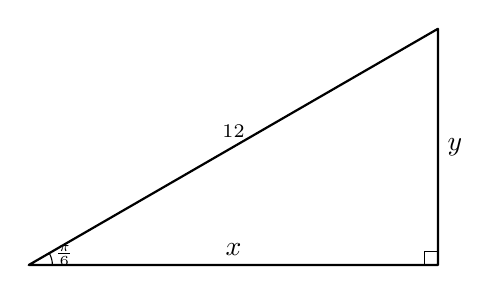
\begin{tikzpicture}[scale=0.5, line cap=round, line join=round]
    % Right triangle: angle pi/6 at origin, hypotenuse 12
    \draw[thick] (0,0) -- (10.392,0) -- (10.392,6) -- cycle;
    \draw (10.392,0) rectangle (10.05,0.35);
    \draw (0,0) ++(0:0.6) arc (0:30:0.6);
    \node[right] at (10.392,3) {$y$};
    \node[above] at (5.2,0) {$x$};
    \node at (0.9,0.25) {\scriptsize $\frac{\pi}{6}$};
    \node[above, sloped] at (5.2,3) {\scriptsize 12};
  \end{tikzpicture}
  \end{center}

  $x = $ \blank

  $y = $ \blank
  \vgappp

  \item A car drives on a circular track with radius 600 feet. A central angle of $\dfrac{7\pi}{6}$ corresponds to 30 seconds. What is the car's average velocity (ft/s) over the first 30 seconds? Exact value, simplest form. \points{3}
  \vgappp

  \item Which angles have the same reference angle? Select all that apply. \points{2}

  \begin{tasks}(1)
    \task $\dfrac{5\pi}{4}$
    \task $\dfrac{13\pi}{6}$
    \task $-\dfrac{7\pi}{4}$
    \task $600^{\circ}$
    \task $-\dfrac{11\pi}{6}$
    \task $\dfrac{7\pi}{3}$
    \task $\dfrac{2\pi}{5}$
    \task $300^{\circ}$
  \end{tasks}
  \vgapp

  \item Evaluate each trigonometric expression. \points{1}

  \begin{center}
  \small
  \begin{tabular}{|l@{\quad}l|}
  \hline
  $\tan(180^{\circ})$: & \blank[3em] \\
  $\sin(240^{\circ})$: & \blank[3em] \\
  $\cos(7\pi/6)$: & \blank[3em] \\
  $\sec(-\pi/4)$: & \blank[3em] \\
  $\tan(120^{\circ})$: & \blank[3em] \\
  $\csc(210^{\circ})$: & \blank[3em] \\
  $\sin(5\pi/3)$: & \blank[3em] \\
  $\cot(3\pi/2)$: & \blank[3em] \\
  $\cos(-2\pi/3)$: & \blank[3em] \\
  \hline
  \end{tabular}
  \end{center}
  \vgapp

  \item If $\tan(\theta) = -\dfrac{3}{4}$ and $\sec(\theta) > 0$, what is $\sin(\theta)$? \points{2}
  \vgappp

  \item Put in order from least to greatest of the followings. \points{3}

  $\sin\bigl(\dfrac{5\pi}{4}\bigr),\ \cos(5\pi),\ \cos(-6\pi), \cdots \\ \sin\bigl(-\dfrac{\pi}{4}\bigr),\ \tan\bigl(\dfrac{\pi}{4}\bigr),\ \cos\bigl(\dfrac{\pi}{9}\bigr)$

  \begin{center}
  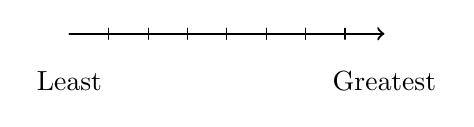
\begin{tikzpicture}[x=0.5cm, line cap=round, line join=round]
    \draw[thick,->] (-4,0) -- (4,0);
    \foreach \k in {-3,-2,...,3} \draw (\k,2pt) -- (\k,-2pt);
    \node[below] at (-4,-0.35) {Least};
    \node[below] at (4,-0.35) {Greatest};
  \end{tikzpicture}
  \end{center}
  \vgapp


  \newpage

  \item \textbf{Part 1:} Fill in the first quadrant of the unit circle (degrees, radians, $(x,y)$). \points{3}

  \begin{center}
  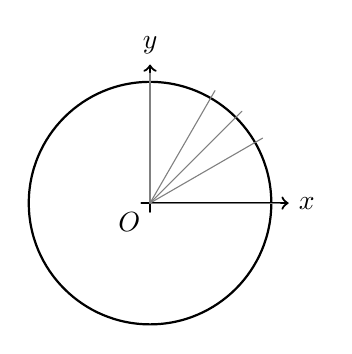
\begin{tikzpicture}[scale=1.1, line cap=round, line join=round]
    \draw[thick] (0,0) circle (1.4);
    \draw[thick,->] (-0.1,0) -- (1.6,0) node[right] {$x$};
    \draw[thick,->] (0,-0.1) -- (0,1.6) node[above] {$y$};
    \foreach \a in {0,30,45,60,90} { \draw[gray] (0,0) -- (\a:1.5); }
    \node[below left] at (0,0) {$O$};
  \end{tikzpicture}
  \end{center}
  \vgap

  \item \textbf{Part 2:} If $\sin(\theta) = 0.823$ ($\theta$ in degrees), find: \points{1}

  \begin{tasks}(1)
    \task $\sec(90^{\circ} - \theta)$: \blank
    \task $\sin(-\theta)$: \blank
    \task $\cos(\theta - 90^{\circ})$: \blank
    \task $\csc(\theta)$: \blank
  \end{tasks}
  \vgapp

\end{enumerate}
